\documentclass[xcolor=pdftex,dvipsnames,table]{beamer}
\usetheme{Darmstadt}
\usepackage{etex}
\providecommand\thispdfpagelabel[1]{}
\usepackage[latin1]{inputenc}
\usepackage{amsmath}
\usepackage{amssymb}
\usepackage{amsthm}
\usepackage{listings}
\usepackage{graphics}
\usepackage{framed}
\usepackage{etex}
\usepackage[all]{xy}
\usepackage{xspace,listings,ulem,tikz}
\usepackage[outline]{contour}
\usepackage[absolute,overlay]{textpos}
\usepackage{hhline}
\usepackage[square,sort,comma,numbers]{natbib}
\setbeamertemplate{footline}[frame number]
\tikzset{
    onslide/.code args={<#1>#2}{% http://tex.stackexchange.com/a/6155/16595
        \only<#1>{\pgfkeysalso{#2}}
    },
    hideshow/.style args={<#1><#2>#3}{%
        onslide=<#1>{move to},
        onslide=<#2>{#3}
    }
}
\lstset{
         basicstyle=\footnotesize\ttfamily, % Standardschrift
         %numbers=left,               % Ort der Zeilennummern
         numberstyle=\tiny,          % Stil der Zeilennummern
         %stepnumber=2,               % Abstand zwischen den Zeilennummern
         numbersep=5pt,              % Abstand der Nummern zum Text
         tabsize=2,                  % Groesse von Tabs
         extendedchars=true,         %
         breaklines=true,            % Zeilen werden Umgebrochen
         keywordstyle=\color{red},
 %        keywordstyle=[1]\textbf,    % Stil der Keywords
 %        keywordstyle=[2]\textbf,    %
 %        keywordstyle=[3]\textbf,    %
 %        keywordstyle=[4]\textbf,   \sqrt{\sqrt{}} %
         %stringstyle=\color{white}\ttfamily, % Farbe der String
         showspaces=false,           % Leerzeichen anzeigen ?
         showtabs=false,             % Tabs anzeigen ?
         xleftmargin=3pt,
         framexleftmargin=3pt,
         framexrightmargin=1pt,
         framexbottommargin=3pt,
         language=C++,
         %backgroundcolor=\color{lightgray},
         showstringspaces=false      % Leerzeichen in Strings anzeigen ?        
 }

 \usetikzlibrary{arrows}
 \usepackage{caption}
\DeclareCaptionFont{white}{\color{white}}
\DeclareCaptionFormat{listing}{\colorbox[cmyk]{0.43, 0.35, 0.35,0.01}{\parbox{\textwidth}{\hspace{15pt}#1#2#3}}}
\captionsetup[lstlisting]{format=listing,labelfont=white,textfont=white, singlelinecheck=false, margin=0pt, font={bf,footnotesize}}
\beamertemplatenavigationsymbolsempty
\newcommand{\N}{\ensuremath{\mathbb{N}}} 
\newcommand{\R}{\ensuremath{\mathbb{R}}} 
\newcommand{\RR}{\ensuremath{\mathbb{R}}} 
\newcommand{\C}{\ensuremath{\mathbb{C}}} 
\newcommand{\Q}{\ensuremath{\mathbb{Q}}} 
\newcommand{\Z}{\ensuremath{\mathbb{Z}}} 
\newcommand{\D}{\ensuremath{\mathbb{D}}}
\newcommand{\lb}{\mathrm{lb}}
\newcommand{\dy}{\mathrm{dy}}
\newcommand{\cc}{\texttt{C++}\xspace}
\newcommand{\bin}{\mathrm{bin}}
\newcommand{\irram}{\texttt{iRRAM}\xspace}
\newcommand{\code}[1]{\texttt{#1}}
\newcommand{\sharpp}{\ensuremath{\#\mathcal P}\xspace}
\newcommand{\sharppu}{\ensuremath{\#{\mathcal P}_1}\xspace}
\newcommand{\fp}{\ensuremath{\mathcal{FP}}\xspace}
  \newcommand{\baana}{\code{BA\_ANA}\xspace}
  \newcommand{\anarect}{\code{ANA\_RECT}\xspace}
  \newcommand{\powerseries}{\code{POWERSERIES}\xspace}
  \newcommand{\poly}{\code{POLY}\xspace}
  \newcommand{\func}{\code{FUNC}\xspace}
  \newcommand{\real}{\code{REAL}\xspace}
  \newcommand{\complex}{\code{COMPLEX}\xspace}
  \newcommand{\temp}{\textcolor{red}}
  \newcommand{\seq}{\mathbf}
\newcommand{\fpu}{\ensuremath{\mathcal{FP}_1}\xspace}
\DeclareMathOperator{\dom}{\mathrm{dom}}
\newtheorem{conjecture}{Conjecture} 
\newtheorem{representation1}{Representation 1} 
\newtheorem{representation1b}{Representation 1'} 
\newtheorem{representation2}{Representation 2} 
\title[Computing with Reals]{Computing with Real Numbers}
\author[ H. Thies]{
		Holger Thies 
}
\institute[The University of Tokyo]{
The University of Tokyo
}
\begin{document}
\setbeamercolor{note}{fg=black,bg=lightgray} 
\date{October 5, 2015}
\frame{
\titlepage
}
\begin{frame}
	\begin{beamercolorbox}[sep=8pt,center,shadow=true,rounded=true]{title}
      \usebeamerfont{title}
	Introduction\par%
    \end{beamercolorbox}
\vfill
\end{frame}
\subsection{Introduction}
\begin{frame}
  \frametitle{Introduction}
  \begin{itemize}[<+->]
      \item Computers are often used to solve problems involving the real numbers
      \item Many applications in science and engineering
      \item The set of reals is uncountable
      \item Thus, it is not possible to represent all real numbers finitely
      \item \ldots and there are more real numbers than computer programs
      \item Classically, Computability and Complexity Theory deal only with finite structures (natural numbers, graphs,\ldots)
      \item How can we define computability of real numbers and functions?
  \end{itemize}
\end{frame}
\subsection{Computing on reals}
\begin{frame}
\frametitle{Computable Real Numbers}
  A real number is called computable if it can be approximated up to any desired precision.
  \vfill
  \pause
\begin{minipage}{.45\textwidth}
		\begin{figure}
		\centering
    \vfill
		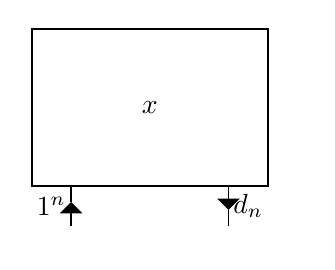
\begin{tikzpicture}<2->
				\path (0,0) rectangle (3.5,-2.7);
			%x
				\draw<2->[thick] (0,0) rectangle (3,-2);
				\node<2-> at (1.5,-1) {$x$};
				\draw<2-> (.5,-2) -- (.5,-2.2);
				\draw<2->[-triangle 90] (.5,-2.5) -- (.5,-2.2);
				\node<2-> at (.25,-2.25) {$1^n$};
				\draw<2->[-triangle 90] (2.5,-2) -- (2.5,-2.3);
				\draw<2-> (2.5,-2.3) -- (2.5,-2.5);
				\node<2-> at (2.75,-2.25) {$d_n$};
				%\node<4-> at (2.85,-2.25) {$d_{n,i}$};
				%\node<4-> at (1.5,-1) {$(a_i)$};
				%\draw<4-> (1,-2) -- (1,-2.2);
				%\draw<4->[-triangle 90] (1,-2.5) -- (1,-2.2);
				%\node<4-> at (1.25,-2.25) {$1^i$};
		\end{tikzpicture}
		\end{figure}
	\end{minipage}
	\hfill
	\begin{minipage}{.45\textwidth}
	\begin{definition}
		A real number $x$ is called computable if there is a computable function $d:\N\to\Z$, such that $ \left|\frac{d(n)}{2^{n+1}} - x\right|\leq 2^{-n}$.   
	\end{definition}
	\end{minipage}
\end{frame}
\begin{frame}
  \frametitle{Non-computable numbers}
  \begin{example}[Specker]
    Let $H \subseteq \N$ be any non-computable subset of the natural numbers (e.g. the Halting problem).
    \pause
    The real number defined by 
    $$
      \sum_{i \in H} 4^{-i}
    $$
    is not computable.
  \end{example}
\end{frame}
\begin{frame}{Polynomial Time Computable Numbers}
  \begin{example}
  $\pi$ is polynomial time computable. \\ \pause
  The Bailey-Borwein-Plouffe formula states
  $$
  \pi = \sum_{k = 0}^{\infty}\left[ \frac{1}{16^k} \left( \frac{4}{8k + 1} - \frac{2}{8k + 4} - \frac{1}{8k + 5} - \frac{1}{8k + 6} \right) \right]
  $$ \pause
  and the error when considering only the first $n$ terms is bounded by $16^{-n}$
  \end{example}
\end{frame}
\subsection{Real functions}

\begin{frame}
  \frametitle{Computable Functions}
	\begin{minipage}{.45\textwidth}
		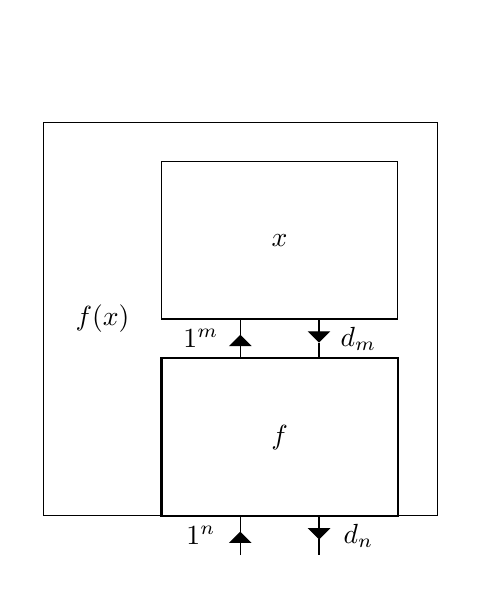
\begin{tikzpicture}
			\path (-1.7,1.7) rectangle (3.7,-5.2);
			%x
				\draw<2-> (0,0) rectangle (3,-2);
				\node<2-> at (1.5,-1) {$x$};
				\draw<2-> (1,-2) -- (1,-2.2);
				\draw<2->[-triangle 90] (1,-2.5) -- (1,-2.2);
				\node<2-> at (.5,-2.25) {$1^m$};
				\draw<2->[-triangle 90] (2,-2) -- (2,-2.3);
				\draw<2-> (2,-2.3) -- (2,-2.5);
				\node<2-> at (2.5,-2.25) {$d_m$};
			%f
				\draw<2->[thick] (0,-2.5) rectangle (3,-4.5);
				\node<2-> at (1.5,-3.5) {$f$};
				\draw<1-> (1,-4.5) -- (1,-4.7);
				\draw<1->[-triangle 90] (1,-5) -- (1,-4.7);
				\node<1-> at (.5,-4.75) {$1^n$};
				\draw<1->[-triangle 90] (2,-4.5) -- (2,-4.8);
				\draw<1-> (2,-4.8) -- (2,-5);
				\node<1-> at (2.5,-4.75) {$d_n$};
			%f(x)
				\draw<1-> (-1.5,.5) rectangle (3.5,-4.5);
				\node<1-> at (-.75,-2) {$f(x)$};
		\end{tikzpicture}
	\end{minipage}
	\hfill
	\begin{minipage}{.47\textwidth}
		\begin{definition}
			\small
			A function $f:[0,1]\to\RR$ is called computable, \newline if there is a machine that,\newline when given oracle access to approximations to the argument $x$,\newline returns approximations to the value $f(x)$.
		\end{definition}
	\end{minipage}
\end{frame}
\begin{frame}[t]{Polynomial Time Computable Functions}
  \begin{example}
  The exponential function $e : [0,1] \to \R$ is polynomial time computable.\pause
  It is
  $$
  e^x = \sum_{n=0}^\infty \frac{x^n}{n!}
  $$\pause
  and
  $$
  \left | \sum_{n=N+1}^\infty \frac{x^n}{n!} \right | \leq 2^{-(N+1)}
  $$
  \end{example}
\end{frame}


\begin{frame}[fragile]{Computable functions are continuous}

\begin{center}

    \begin{tikzpicture}[scale=1.25]
    \draw[red,thick] (0,3) parabola bend (0,3) (2,2.0);
    \draw[red,thick] (2,1.0) parabola bend (2,1.0) (4, 3.0); 
    \draw[red, fill=white] (2,2.0) circle (.1cm); 
    \draw[fill=blue] (2,1.0) circle (.1cm); 
    %\draw[loosely dotted] (0,0) grid (4,4);
    %\path[use as bounding box] (-2,-1) rectangle (5,5);
    \draw[->] (-0.2,0) -- (4.25,0) node[right] {$x$};
    \draw[->] (0,-0.25) -- (0,4.25) node[above] {$y$};
    \foreach \x/\xtext in {1/1, 2/2, 3/3}
    \draw[shift={(\x,0)}] (0pt,2pt) -- (0pt,-2pt) node[below] {};
    \foreach \y/\ytext in {1/1, 2/2, 3/3, 4/4}
    \draw[shift={(0,\y)}] (2pt,0pt) -- (-2pt,0pt) node[left] {};
   % \draw[dotted,line width=2pt] (0,1) -- (2,1);
    %\draw[dotted,line width=2pt] (2,1) -- (2,0);
    %\draw[dotted,line width=2pt] (0,2.21) -- (1.8,2.21);
    \%draw[dotted,line width=2pt] (1.8,2.21) -- (1.8,0);
    %\draw[green,line width=3pt] (0,0.5) -- (0,2.5);
    %\draw[green,line width=3pt] (4pt,0.5) -- (-4pt,0.5);
    %\draw[green,line width=3pt] (4pt,2.5) -- (-4pt,2.5);
    %\draw[green,line width=3pt] (0,0.5) -- (0,1.5);
    %\draw[green,line width=3pt] (4pt,0.5) -- (-4pt,0.5);
    %\draw[green,line width=3pt] (4pt,1.5) -- (-4pt,1.5);

%    \draw[blue,line width=3pt] (0.5,0) -- (3.5,0);
%   \draw[blue,line width=3pt] (0.5,4pt) -- (0.5,-4pt);
 %   \draw[blue,line width=3pt] (3.5,4pt) -- (3.5,-4pt);
 %     \draw[blue,line width=3pt] (1.0,0) -- (3.0,0);
   % \draw[blue,line width=3pt] (1.0,4pt) -- (1.0,-4pt);
   % \draw[blue,line width=3pt] (3.0,4pt) -- (3.0,-4pt);  
   %   \draw[blue,line width=3pt] (1.5,0) -- (2.5,0);
   % \draw[blue,line width=3pt] (1.5,4pt) -- (1.5,-4pt);
   % \draw[blue,line width=3pt] (2.5,4pt) -- (2.5,-4pt);  
%
    \end{tikzpicture}
\end{center}
\end{frame}

\addtocounter{framenumber}{-1}
\begin{frame}[fragile]{Computable functions are continuous}

\begin{center}

    \begin{tikzpicture}[scale=1.25]
    \draw[red,thick] (0,3) parabola bend (0,3) (2,2.0);
    \draw[red,thick] (2,1.0) parabola bend (2,1.0) (4, 3.0); 
    \draw[red, fill=white] (2,2.0) circle (.1cm); 
    \draw[fill=blue] (2,1.0) circle (.1cm); 
    %\draw[loosely dotted] (0,0) grid (4,4);
    %\path[use as bounding box] (-2,-1) rectangle (5,5);
    \draw[->] (-0.2,0) -- (4.25,0) node[right] {$x$};
    \draw[->] (0,-0.25) -- (0,4.25) node[above] {$y$};
    \foreach \x/\xtext in {1/1, 2/2, 3/3}
    \draw[shift={(\x,0)}] (0pt,2pt) -- (0pt,-2pt) node[below] {};
    \foreach \y/\ytext in {1/1, 2/2, 3/3, 4/4}
    \draw[shift={(0,\y)}] (2pt,0pt) -- (-2pt,0pt) node[left] {};
    \draw[dotted,line width=2pt] (0,1) -- (2,1);
    \draw[dotted,line width=2pt] (2,1) -- (2,0);
    %\draw[dotted,line width=2pt] (0,2.21) -- (1.8,2.21);
    \%draw[dotted,line width=2pt] (1.8,2.21) -- (1.8,0);
    %\draw[green,line width=3pt] (0,0.5) -- (0,2.5);
    %\draw[green,line width=3pt] (4pt,0.5) -- (-4pt,0.5);
    %\draw[green,line width=3pt] (4pt,2.5) -- (-4pt,2.5);
    %\draw[green,line width=3pt] (0,0.5) -- (0,1.5);
    %\draw[green,line width=3pt] (4pt,0.5) -- (-4pt,0.5);
    %\draw[green,line width=3pt] (4pt,1.5) -- (-4pt,1.5);

%    \draw[blue,line width=3pt] (0.5,0) -- (3.5,0);
%   \draw[blue,line width=3pt] (0.5,4pt) -- (0.5,-4pt);
 %   \draw[blue,line width=3pt] (3.5,4pt) -- (3.5,-4pt);
 %     \draw[blue,line width=3pt] (1.0,0) -- (3.0,0);
   % \draw[blue,line width=3pt] (1.0,4pt) -- (1.0,-4pt);
   % \draw[blue,line width=3pt] (3.0,4pt) -- (3.0,-4pt);  
   %   \draw[blue,line width=3pt] (1.5,0) -- (2.5,0);
   % \draw[blue,line width=3pt] (1.5,4pt) -- (1.5,-4pt);
   % \draw[blue,line width=3pt] (2.5,4pt) -- (2.5,-4pt);  
%
    \end{tikzpicture}
\end{center}
\end{frame}

\addtocounter{framenumber}{-1}
\begin{frame}[fragile]{Computable functions are continuous}

\begin{center}

    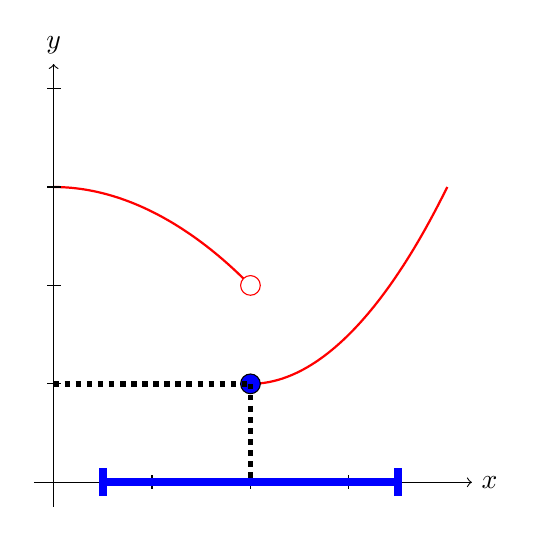
\begin{tikzpicture}[scale=1.25]
    \draw[red,thick] (0,3) parabola bend (0,3) (2,2.0);
    \draw[red,thick] (2,1.0) parabola bend (2,1.0) (4, 3.0); 
    \draw[red, fill=white] (2,2.0) circle (.1cm); 
    \draw[fill=blue] (2,1.0) circle (.1cm); 
    %\draw[loosely dotted] (0,0) grid (4,4);
    %\path[use as bounding box] (-2,-1) rectangle (5,5);
    \draw[->] (-0.2,0) -- (4.25,0) node[right] {$x$};
    \draw[->] (0,-0.25) -- (0,4.25) node[above] {$y$};
    \foreach \x/\xtext in {1/1, 2/2, 3/3}
    \draw[shift={(\x,0)}] (0pt,2pt) -- (0pt,-2pt) node[below] {};
    \foreach \y/\ytext in {1/1, 2/2, 3/3, 4/4}
    \draw[shift={(0,\y)}] (2pt,0pt) -- (-2pt,0pt) node[left] {};
    \draw[dotted,line width=2pt] (0,1) -- (2,1);
    \draw[dotted,line width=2pt] (2,1) -- (2,0);
    %\draw[dotted,line width=2pt] (0,2.21) -- (1.8,2.21);
    \%draw[dotted,line width=2pt] (1.8,2.21) -- (1.8,0);
    %\draw[green,line width=3pt] (0,0.5) -- (0,2.5);
    %\draw[green,line width=3pt] (4pt,0.5) -- (-4pt,0.5);
    %\draw[green,line width=3pt] (4pt,2.5) -- (-4pt,2.5);
    %\draw[green,line width=3pt] (0,0.5) -- (0,1.5);
    %\draw[green,line width=3pt] (4pt,0.5) -- (-4pt,0.5);
    %\draw[green,line width=3pt] (4pt,1.5) -- (-4pt,1.5);

    \draw[blue,line width=3pt] (0.5,0) -- (3.5,0);
   \draw[blue,line width=3pt] (0.5,4pt) -- (0.5,-4pt);
    \draw[blue,line width=3pt] (3.5,4pt) -- (3.5,-4pt);
 %     \draw[blue,line width=3pt] (1.0,0) -- (3.0,0);
   % \draw[blue,line width=3pt] (1.0,4pt) -- (1.0,-4pt);
   % \draw[blue,line width=3pt] (3.0,4pt) -- (3.0,-4pt);  
   %   \draw[blue,line width=3pt] (1.5,0) -- (2.5,0);
   % \draw[blue,line width=3pt] (1.5,4pt) -- (1.5,-4pt);
   % \draw[blue,line width=3pt] (2.5,4pt) -- (2.5,-4pt);  
%
    \end{tikzpicture}
\end{center}
\end{frame}


\addtocounter{framenumber}{-1}
\begin{frame}[fragile]{Computable functions are continuous}

\begin{center}

    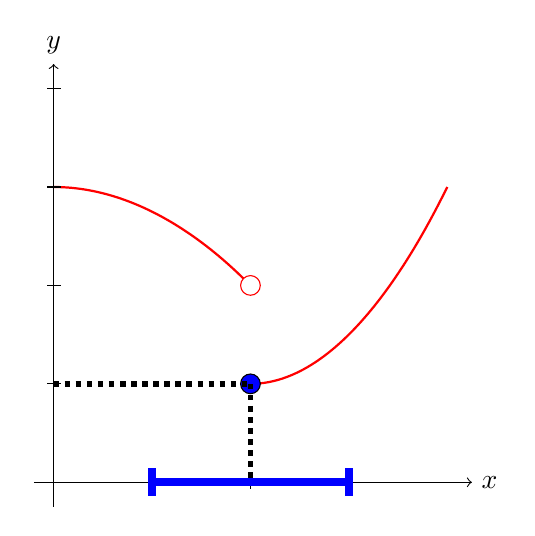
\begin{tikzpicture}[scale=1.25]
    \draw[red,thick] (0,3) parabola bend (0,3) (2,2.0);
    \draw[red,thick] (2,1.0) parabola bend (2,1.0) (4, 3.0); 
    \draw[red, fill=white] (2,2.0) circle (.1cm); 
    \draw[fill=blue] (2,1.0) circle (.1cm); 
    %\draw[loosely dotted] (0,0) grid (4,4);
    %\path[use as bounding box] (-2,-1) rectangle (5,5);
    \draw[->] (-0.2,0) -- (4.25,0) node[right] {$x$};
    \draw[->] (0,-0.25) -- (0,4.25) node[above] {$y$};
    \foreach \x/\xtext in {1/1, 2/2, 3/3}
    \draw[shift={(\x,0)}] (0pt,2pt) -- (0pt,-2pt) node[below] {};
    \foreach \y/\ytext in {1/1, 2/2, 3/3, 4/4}
    \draw[shift={(0,\y)}] (2pt,0pt) -- (-2pt,0pt) node[left] {};
    \draw[dotted,line width=2pt] (0,1) -- (2,1);
    \draw[dotted,line width=2pt] (2,1) -- (2,0);
    %\draw[dotted,line width=2pt] (0,2.21) -- (1.8,2.21);
    \%draw[dotted,line width=2pt] (1.8,2.21) -- (1.8,0);
    %\draw[green,line width=3pt] (0,0.5) -- (0,2.5);
    %\draw[green,line width=3pt] (4pt,0.5) -- (-4pt,0.5);
    %\draw[green,line width=3pt] (4pt,2.5) -- (-4pt,2.5);
    %\draw[green,line width=3pt] (0,0.5) -- (0,1.5);
    %\draw[green,line width=3pt] (4pt,0.5) -- (-4pt,0.5);
    %\draw[green,line width=3pt] (4pt,1.5) -- (-4pt,1.5);

%    \draw[blue,line width=3pt] (0.5,0) -- (3.5,0);
 %  \draw[blue,line width=3pt] (0.5,4pt) -- (0.5,-4pt);
  %  \draw[blue,line width=3pt] (3.5,4pt) -- (3.5,-4pt);
      \draw[blue,line width=3pt] (1.0,0) -- (3.0,0);
    \draw[blue,line width=3pt] (1.0,4pt) -- (1.0,-4pt);
    \draw[blue,line width=3pt] (3.0,4pt) -- (3.0,-4pt);  
   %   \draw[blue,line width=3pt] (1.5,0) -- (2.5,0);
   % \draw[blue,line width=3pt] (1.5,4pt) -- (1.5,-4pt);
   % \draw[blue,line width=3pt] (2.5,4pt) -- (2.5,-4pt);  
%
    \end{tikzpicture}
\end{center}
\end{frame}



\addtocounter{framenumber}{-1}
\begin{frame}[fragile]{Computable functions are continuous}

\begin{center}

    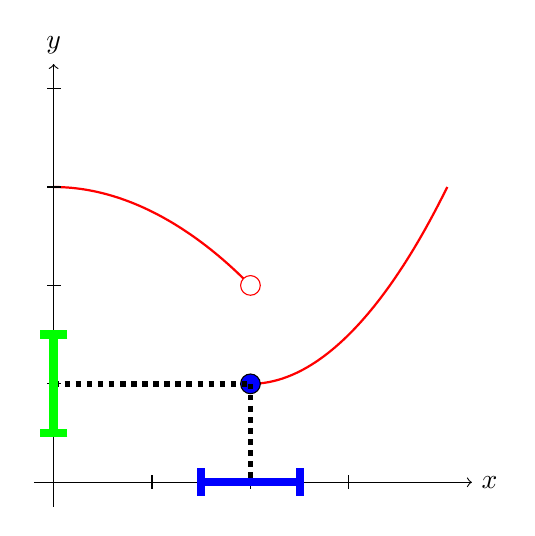
\begin{tikzpicture}[scale=1.25]
    \draw[red,thick] (0,3) parabola bend (0,3) (2,2.0);
    \draw[red,thick] (2,1.0) parabola bend (2,1.0) (4, 3.0); 
    \draw[red, fill=white] (2,2.0) circle (.1cm); 
    \draw[fill=blue] (2,1.0) circle (.1cm); 
    %\draw[loosely dotted] (0,0) grid (4,4);
    %\path[use as bounding box] (-2,-1) rectangle (5,5);
    \draw[->] (-0.2,0) -- (4.25,0) node[right] {$x$};
    \draw[->] (0,-0.25) -- (0,4.25) node[above] {$y$};
    \foreach \x/\xtext in {1/1, 2/2, 3/3}
    \draw[shift={(\x,0)}] (0pt,2pt) -- (0pt,-2pt) node[below] {};
    \foreach \y/\ytext in {1/1, 2/2, 3/3, 4/4}
    \draw[shift={(0,\y)}] (2pt,0pt) -- (-2pt,0pt) node[left] {};
    \draw[dotted,line width=2pt] (0,1) -- (2,1);
    \draw[dotted,line width=2pt] (2,1) -- (2,0);
    %\draw[dotted,line width=2pt] (0,2.21) -- (1.8,2.21);
    \%draw[dotted,line width=2pt] (1.8,2.21) -- (1.8,0);
    %\draw[green,line width=3pt] (0,0.5) -- (0,2.5);
    %\draw[green,line width=3pt] (4pt,0.5) -- (-4pt,0.5);
    %\draw[green,line width=3pt] (4pt,2.5) -- (-4pt,2.5);
    \draw[green,line width=3pt] (0,0.5) -- (0,1.5);
    \draw[green,line width=3pt] (4pt,0.5) -- (-4pt,0.5);
    \draw[green,line width=3pt] (4pt,1.5) -- (-4pt,1.5);

%    \draw[blue,line width=3pt] (0.5,0) -- (3.5,0);
 %  \draw[blue,line width=3pt] (0.5,4pt) -- (0.5,-4pt);
  %  \draw[blue,line width=3pt] (3.5,4pt) -- (3.5,-4pt);
 %     \draw[blue,line width=3pt] (1.0,0) -- (3.0,0);
  %  \draw[blue,line width=3pt] (1.0,4pt) -- (1.0,-4pt);
  %  \draw[blue,line width=3pt] (3.0,4pt) -- (3.0,-4pt);  
      \draw[blue,line width=3pt] (1.5,0) -- (2.5,0);
    \draw[blue,line width=3pt] (1.5,4pt) -- (1.5,-4pt);
    \draw[blue,line width=3pt] (2.5,4pt) -- (2.5,-4pt);  
%
    \end{tikzpicture}
\end{center}
\end{frame}

\addtocounter{framenumber}{-1}
\begin{frame}[fragile]{Computable functions are continuous}

\begin{center}

    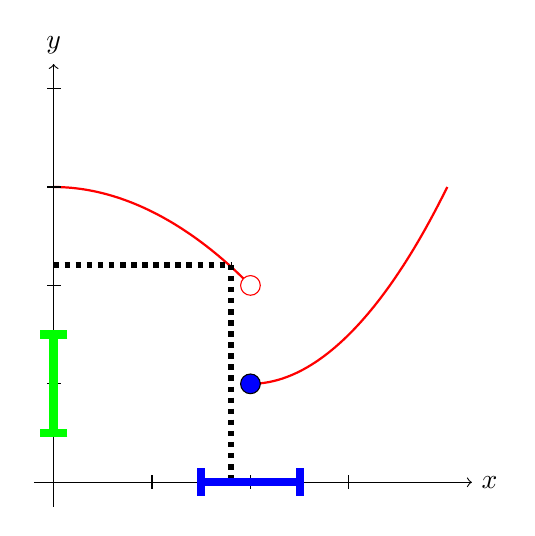
\begin{tikzpicture}[scale=1.25]
    \draw[red,thick] (0,3) parabola bend (0,3) (2,2.0);
    \draw[red,thick] (2,1.0) parabola bend (2,1.0) (4, 3.0); 
    \draw[red, fill=white] (2,2.0) circle (.1cm); 
    \draw[fill=blue] (2,1.0) circle (.1cm); 
    %\draw[loosely dotted] (0,0) grid (4,4);
    %\path[use as bounding box] (-2,-1) rectangle (5,5);
    \draw[->] (-0.2,0) -- (4.25,0) node[right] {$x$};
    \draw[->] (0,-0.25) -- (0,4.25) node[above] {$y$};
    \foreach \x/\xtext in {1/1, 2/2, 3/3}
    \draw[shift={(\x,0)}] (0pt,2pt) -- (0pt,-2pt) node[below] {};
    \foreach \y/\ytext in {1/1, 2/2, 3/3, 4/4}
    \draw[shift={(0,\y)}] (2pt,0pt) -- (-2pt,0pt) node[left] {};
    %\draw[dotted,line width=2pt] (0,1) -- (2,1);
    %\draw[dotted,line width=2pt] (2,1) -- (2,0);
    \draw[dotted,line width=2pt] (0,2.21) -- (1.8,2.21);
    \draw[dotted,line width=2pt] (1.8,2.21) -- (1.8,0);
    %\draw[green,line width=3pt] (0,0.5) -- (0,2.5);
    %\draw[green,line width=3pt] (4pt,0.5) -- (-4pt,0.5);
    %\draw[green,line width=3pt] (4pt,2.5) -- (-4pt,2.5);
   \draw[green,line width=3pt] (0,0.5) -- (0,1.5);
    \draw[green,line width=3pt] (4pt,0.5) -- (-4pt,0.5);
    \draw[green,line width=3pt] (4pt,1.5) -- (-4pt,1.5);

%    \draw[blue,line width=3pt] (0.5,0) -- (3.5,0);
 %  \draw[blue,line width=3pt] (0.5,4pt) -- (0.5,-4pt);
  %  \draw[blue,line width=3pt] (3.5,4pt) -- (3.5,-4pt);
 %     \draw[blue,line width=3pt] (1.0,0) -- (3.0,0);
  %  \draw[blue,line width=3pt] (1.0,4pt) -- (1.0,-4pt);
  %  \draw[blue,line width=3pt] (3.0,4pt) -- (3.0,-4pt);  
      \draw[blue,line width=3pt] (1.5,0) -- (2.5,0);
    \draw[blue,line width=3pt] (1.5,4pt) -- (1.5,-4pt);
    \draw[blue,line width=3pt] (2.5,4pt) -- (2.5,-4pt);  
%
    \end{tikzpicture}
\end{center}
\end{frame}


\addtocounter{framenumber}{-1}
\begin{frame}[fragile]{Computable functions are continuous}

\begin{center}

    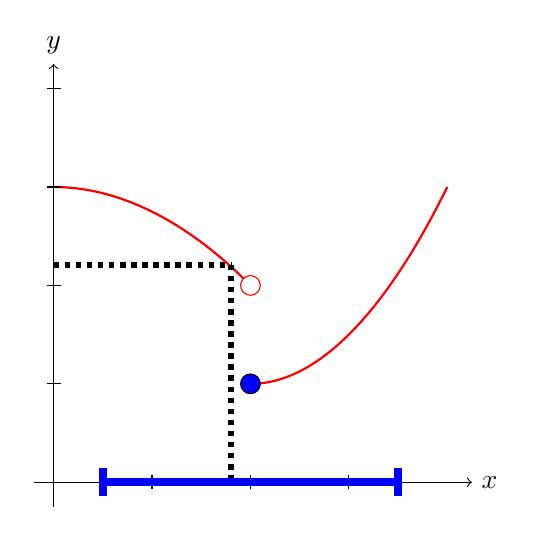
\begin{tikzpicture}[scale=1.25]
    \draw[red,thick] (0,3) parabola bend (0,3) (2,2.0);
    \draw[red,thick] (2,1.0) parabola bend (2,1.0) (4, 3.0); 
    \draw[red, fill=white] (2,2.0) circle (.1cm); 
    \draw[fill=blue] (2,1.0) circle (.1cm); 
    %\draw[loosely dotted] (0,0) grid (4,4);
    %\path[use as bounding box] (-2,-1) rectangle (5,5);
    \draw[->] (-0.2,0) -- (4.25,0) node[right] {$x$};
    \draw[->] (0,-0.25) -- (0,4.25) node[above] {$y$};
    \foreach \x/\xtext in {1/1, 2/2, 3/3}
    \draw[shift={(\x,0)}] (0pt,2pt) -- (0pt,-2pt) node[below] {};
    \foreach \y/\ytext in {1/1, 2/2, 3/3, 4/4}
    \draw[shift={(0,\y)}] (2pt,0pt) -- (-2pt,0pt) node[left] {};
    %\draw[dotted,line width=2pt] (0,1) -- (2,1);
    %\draw[dotted,line width=2pt] (2,1) -- (2,0);
    \draw[dotted,line width=2pt] (0,2.21) -- (1.8,2.21);
    \draw[dotted,line width=2pt] (1.8,2.21) -- (1.8,0);
    %\draw[green,line width=3pt] (0,0.5) -- (0,2.5);
    %\draw[green,line width=3pt] (4pt,0.5) -- (-4pt,0.5);
    %\draw[green,line width=3pt] (4pt,2.5) -- (-4pt,2.5);
    %\draw[green,line width=3pt] (0,0.5) -- (0,1.5);
    %\draw[green,line width=3pt] (4pt,0.5) -- (-4pt,0.5);
    %\draw[green,line width=3pt] (4pt,1.5) -- (-4pt,1.5);

    \draw[blue,line width=3pt] (0.5,0) -- (3.5,0);
   \draw[blue,line width=3pt] (0.5,4pt) -- (0.5,-4pt);
    \draw[blue,line width=3pt] (3.5,4pt) -- (3.5,-4pt);
 %     \draw[blue,line width=3pt] (1.0,0) -- (3.0,0);
   % \draw[blue,line width=3pt] (1.0,4pt) -- (1.0,-4pt);
   % \draw[blue,line width=3pt] (3.0,4pt) -- (3.0,-4pt);  
   %   \draw[blue,line width=3pt] (1.5,0) -- (2.5,0);
   % \draw[blue,line width=3pt] (1.5,4pt) -- (1.5,-4pt);
   % \draw[blue,line width=3pt] (2.5,4pt) -- (2.5,-4pt);  
%
    \end{tikzpicture}
\end{center}
\end{frame}


\addtocounter{framenumber}{-1}
\begin{frame}[fragile]{Computable functions are continuous}

\begin{center}

    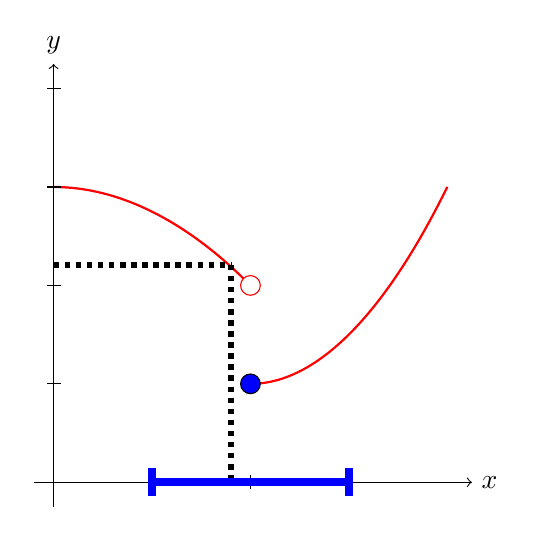
\begin{tikzpicture}[scale=1.25]
    \draw[red,thick] (0,3) parabola bend (0,3) (2,2.0);
    \draw[red,thick] (2,1.0) parabola bend (2,1.0) (4, 3.0); 
    \draw[red, fill=white] (2,2.0) circle (.1cm); 
    \draw[fill=blue] (2,1.0) circle (.1cm); 
    %\draw[loosely dotted] (0,0) grid (4,4);
    %\path[use as bounding box] (-2,-1) rectangle (5,5);
    \draw[->] (-0.2,0) -- (4.25,0) node[right] {$x$};
    \draw[->] (0,-0.25) -- (0,4.25) node[above] {$y$};
    \foreach \x/\xtext in {1/1, 2/2, 3/3}
    \draw[shift={(\x,0)}] (0pt,2pt) -- (0pt,-2pt) node[below] {};
    \foreach \y/\ytext in {1/1, 2/2, 3/3, 4/4}
    \draw[shift={(0,\y)}] (2pt,0pt) -- (-2pt,0pt) node[left] {};
    %\draw[dotted,line width=2pt] (0,1) -- (2,1);
    %\draw[dotted,line width=2pt] (2,1) -- (2,0);
    \draw[dotted,line width=2pt] (0,2.21) -- (1.8,2.21);
    \draw[dotted,line width=2pt] (1.8,2.21) -- (1.8,0);
    %\draw[green,line width=3pt] (0,0.5) -- (0,2.5);
    %\draw[green,line width=3pt] (4pt,0.5) -- (-4pt,0.5);
    %\draw[green,line width=3pt] (4pt,2.5) -- (-4pt,2.5);
    %\draw[green,line width=3pt] (0,0.5) -- (0,1.5);
    %\draw[green,line width=3pt] (4pt,0.5) -- (-4pt,0.5);
    %\draw[green,line width=3pt] (4pt,1.5) -- (-4pt,1.5);

%    \draw[blue,line width=3pt] (0.5,0) -- (3.5,0);
 %  \draw[blue,line width=3pt] (0.5,4pt) -- (0.5,-4pt);
  %  \draw[blue,line width=3pt] (3.5,4pt) -- (3.5,-4pt);
      \draw[blue,line width=3pt] (1.0,0) -- (3.0,0);
    \draw[blue,line width=3pt] (1.0,4pt) -- (1.0,-4pt);
    \draw[blue,line width=3pt] (3.0,4pt) -- (3.0,-4pt);  
   %   \draw[blue,line width=3pt] (1.5,0) -- (2.5,0);
   % \draw[blue,line width=3pt] (1.5,4pt) -- (1.5,-4pt);
   % \draw[blue,line width=3pt] (2.5,4pt) -- (2.5,-4pt);  
%
    \end{tikzpicture}
\end{center}
\end{frame}

\addtocounter{framenumber}{-1}
\begin{frame}[fragile]{Computable functions are continuous}

\begin{center}

    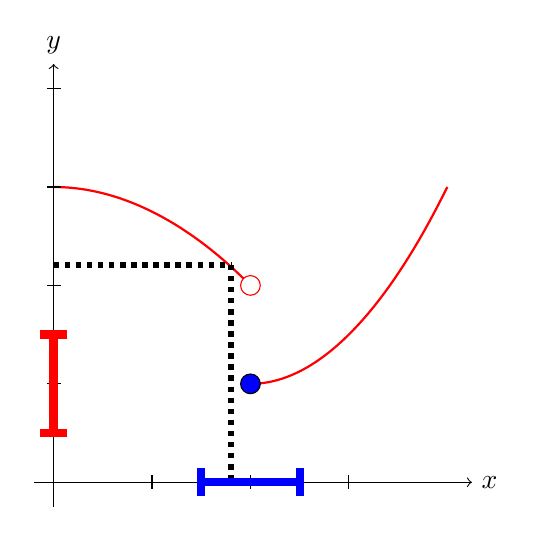
\begin{tikzpicture}[scale=1.25]
    \draw[red,thick] (0,3) parabola bend (0,3) (2,2.0);
    \draw[red,thick] (2,1.0) parabola bend (2,1.0) (4, 3.0); 
    \draw[red, fill=white] (2,2.0) circle (.1cm); 
    \draw[fill=blue] (2,1.0) circle (.1cm); 
    %\draw[loosely dotted] (0,0) grid (4,4);
    %\path[use as bounding box] (-2,-1) rectangle (5,5);
    \draw[->] (-0.2,0) -- (4.25,0) node[right] {$x$};
    \draw[->] (0,-0.25) -- (0,4.25) node[above] {$y$};
    \foreach \x/\xtext in {1/1, 2/2, 3/3}
    \draw[shift={(\x,0)}] (0pt,2pt) -- (0pt,-2pt) node[below] {};
    \foreach \y/\ytext in {1/1, 2/2, 3/3, 4/4}
    \draw[shift={(0,\y)}] (2pt,0pt) -- (-2pt,0pt) node[left] {};
    %\draw[dotted,line width=2pt] (0,1) -- (2,1);
    %\draw[dotted,line width=2pt] (2,1) -- (2,0);
    \draw[dotted,line width=2pt] (0,2.21) -- (1.8,2.21);
    \draw[dotted,line width=2pt] (1.8,2.21) -- (1.8,0);
    %\draw[green,line width=3pt] (0,0.5) -- (0,2.5);
    %\draw[green,line width=3pt] (4pt,0.5) -- (-4pt,0.5);
    %\draw[green,line width=3pt] (4pt,2.5) -- (-4pt,2.5);
    \draw[red,line width=3pt] (0,0.5) -- (0,1.5);
    \draw[red,line width=3pt] (4pt,0.5) -- (-4pt,0.5);
    \draw[red,line width=3pt] (4pt,1.5) -- (-4pt,1.5);

%    \draw[blue,line width=3pt] (0.5,0) -- (3.5,0);
 %  \draw[blue,line width=3pt] (0.5,4pt) -- (0.5,-4pt);
  %  \draw[blue,line width=3pt] (3.5,4pt) -- (3.5,-4pt);
 %     \draw[blue,line width=3pt] (1.0,0) -- (3.0,0);
  %  \draw[blue,line width=3pt] (1.0,4pt) -- (1.0,-4pt);
  %  \draw[blue,line width=3pt] (3.0,4pt) -- (3.0,-4pt);  
      \draw[blue,line width=3pt] (1.5,0) -- (2.5,0);
    \draw[blue,line width=3pt] (1.5,4pt) -- (1.5,-4pt);
    \draw[blue,line width=3pt] (2.5,4pt) -- (2.5,-4pt);  
%
    \end{tikzpicture}
\end{center}
\end{frame}

\addtocounter{framenumber}{-1}
\begin{frame}[fragile]{Computable functions are continuous}

\begin{center}

    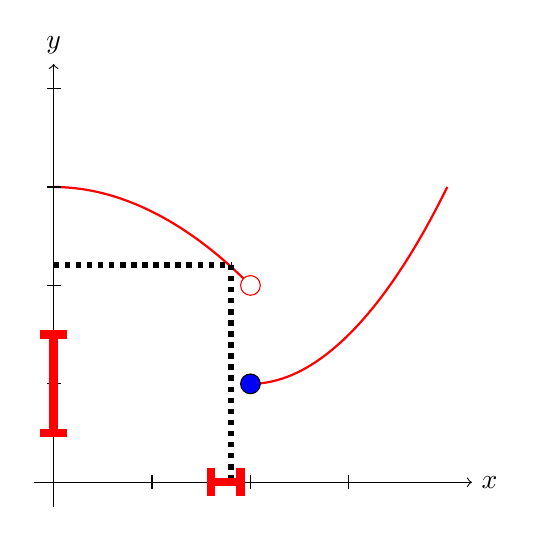
\begin{tikzpicture}[scale=1.25]
    \draw[red,thick] (0,3) parabola bend (0,3) (2,2.0);
    \draw[red,thick] (2,1.0) parabola bend (2,1.0) (4, 3.0); 
    \draw[red, fill=white] (2,2.0) circle (.1cm); 
    \draw[fill=blue] (2,1.0) circle (.1cm); 
    %\draw[loosely dotted] (0,0) grid (4,4);
    %\path[use as bounding box] (-2,-1) rectangle (5,5);
    \draw[->] (-0.2,0) -- (4.25,0) node[right] {$x$};
    \draw[->] (0,-0.25) -- (0,4.25) node[above] {$y$};
    \foreach \x/\xtext in {1/1, 2/2, 3/3}
    \draw[shift={(\x,0)}] (0pt,2pt) -- (0pt,-2pt) node[below] {};
    \foreach \y/\ytext in {1/1, 2/2, 3/3, 4/4}
    \draw[shift={(0,\y)}] (2pt,0pt) -- (-2pt,0pt) node[left] {};
    %\draw[dotted,line width=2pt] (0,1) -- (2,1);
    %\draw[dotted,line width=2pt] (2,1) -- (2,0);
    \draw[dotted,line width=2pt] (0,2.21) -- (1.8,2.21);
    \draw[dotted,line width=2pt] (1.8,2.21) -- (1.8,0);
    %\draw[green,line width=3pt] (0,0.5) -- (0,2.5);
    %\draw[green,line width=3pt] (4pt,0.5) -- (-4pt,0.5);
    %\draw[green,line width=3pt] (4pt,2.5) -- (-4pt,2.5);
    \draw[red,line width=3pt] (0,0.5) -- (0,1.5);
    \draw[red,line width=3pt] (4pt,0.5) -- (-4pt,0.5);
    \draw[red,line width=3pt] (4pt,1.5) -- (-4pt,1.5);

%    \draw[blue,line width=3pt] (0.5,0) -- (3.5,0);
 %  \draw[blue,line width=3pt] (0.5,4pt) -- (0.5,-4pt);
  %  \draw[blue,line width=3pt] (3.5,4pt) -- (3.5,-4pt);
 %     \draw[blue,line width=3pt] (1.0,0) -- (3.0,0);
  %  \draw[blue,line width=3pt] (1.0,4pt) -- (1.0,-4pt);
  %  \draw[blue,line width=3pt] (3.0,4pt) -- (3.0,-4pt);  
      \draw[red,line width=3pt] (1.6,0) -- (1.9,0);
    \draw[red,line width=3pt] (1.6,4pt) -- (1.6,-4pt);
    \draw[red,line width=3pt] (1.9,4pt) -- (1.9,-4pt);  
%
    \end{tikzpicture}
\end{center}
\end{frame}



\begin{frame}
	\begin{beamercolorbox}[sep=8pt,center,shadow=true,rounded=true]{title}
      \usebeamerfont{title}
	Computable Reals in Practice\par%
    \end{beamercolorbox}
\vfill
\end{frame}
\subsection{Overview}
\begin{frame}
  \frametitle{Overview}
  Different approaches to compute with real numbers on a computer
  \begin{itemize}[<+->]
      \item Floating-Point Arithmetic
      \item Arbitrary-Precision Arithmetic
      \item Interval Arithmetic
      \item Symbolic Computation
      \item \textbf{Exact Real Arithmetic}
  \end{itemize}
\end{frame}
\subsection{Exact Real Arithmetic}
\begin{frame}[<+->][t,fragile]
    \frametitle{Computations via DAGs: Top-Down Approach}
  \begin{lstlisting}
    x = sqrt(x0)+(x1*x2);
  \end{lstlisting}
  \vspace{20pt}
  \begin{center}
        \begin{tikzpicture}[remember picture, overlay
            ,->,shorten >=1pt,auto,node distance=2.5cm,minimum
              size=0.8cm,main node/.style={circle,fill=yellow!20,draw,font=\sffamily\small}]
    
    \node<2->[main node] (1) {$+$};
    \node<2->[main node] (2) [below left of=1] {$\sqrt{}$};
    \node<2->[main node] (6) [below left of=2] {$x_0$};
    \node<2->[main node] (3) [below right of=1] {$\times$};
    \node<2->[main node] (4) [below left of=3] {$x_1$};
    \node<2->[main node] (5) [below right of=3] {$x_2$};

    \node<3->[color=red] at (0.0,0.7) {$2^{-n}$};
    \node<4->[color=red] at (-2.0,-1.1) {$2^{-(n+1)}$};
    \node<4->[color=red] at (2.0,-1.1) {$2^{-(n+1)}$};
    \node<5->[color=red] at (-4.0,-2.6) {$2^{-(n+2)}$};
    \node<5->[color=red] at (-0.0,-2.8) {$2^{-(n+3)}$};
    \node<5->[color=red] at (4.0,-2.8) {$2^{-(n+3)}$};
    \path<2->[every node/.style={font=\sffamily\small}]
    (1) edge (2)
    (2) edge (6)
    (1) edge (3)
    (3) edge (4)
    (3) edge (5);
  \end{tikzpicture}
\end{center}
\end{frame}
\begin{frame}[<+->][fragile]
  \frametitle{Computations via DAGs: Top-Down Approach}
  \begin{textblock*}{\paperwidth}(-20pt,60pt)
        \raggedright
      \begin{lstlisting}
        y = x[0];
        for(int i=1; i<=1000; i++)
          y += x[i];
        \end{lstlisting}
        \hspace{.5em}
  \end{textblock*}
  \vfill
  \begin{center}
    \onslide<2->{
      \begin{tikzpicture}[remember picture, overlay,
          ->,shorten >=1pt,auto,node distance=2.4cm,minimum
            size=0.8cm,main node/.style={circle,fill=yellow!20,draw,font=\sffamily\small}]
    \node[main node] (1) {$+$};
    \node[main node] (2) [below left of=1] {$x_0$};
    \node[main node] (3) [below right of=1] {$x_1$};
    \node[main node] (4) [above right of=1] {$+$};
    \node[minimum size=0.5cm] (8) at (0.9, 0.9) {$\cdots$};
    \node[main node,font=\sffamily\tiny] (5) [below right of=4] {$x_{999}$};
    \node[main node] (6) [above right of=4] {$+$};
    \node[main node] (7) [below right of=6] {$x_{N}$};
    \node<3->[color=red] at (3.5,4.2) {$2^{-n}$};
    \node<4->[color=red] at (1.7,2.4) {$2^{-(n+1)}$};
    \node<4->[color=red] at (5.4,2.4) {$2^{-(n+1)}$};
    \node<4->[color=red] at (3.5,0.8) {$2^{-(n+2)}$};
    \node<4->[color=red] at (0.0,0.8) {$2^{-(n+999)}$};
    \node<5->[color=red] at (1.5,-1.2) {$2^{-(n+1000)}$};
    \node<5->[color=red] at (-2.0,-1.2) {$2^{-(n+1000)}$};
    \path[every node/.style={font=\sffamily\small}]
    (1) edge (2)
    (1) edge (3)
    (4) edge (5)
    (6) edge (4)
    (4) edge (8)
    (8) edge (1)
    (6) edge (7);
  \end{tikzpicture}
  }
  \end{center}
\end{frame}
\begin{frame}[fragile]
  \frametitle{Computations via DAGs: Bottom-Up Approach}
  \begin{textblock*}{\paperwidth}(-20pt,60pt)
        \raggedright
      \begin{lstlisting}
        y = x[0];
        for(int i=1; i<=1000; i++)
          y += x[i];
        \end{lstlisting}
        \hspace{.5em}
  \end{textblock*}
    \vfill
    \begin{center}
      \begin{tikzpicture}[remember picture, overlay,
            ->,shorten >=1pt,auto,node distance=2.5cm,minimum
              size=0.8cm,main node/.style={circle,fill=yellow!20,draw,font=\sffamily\small}]
      \node[main node] (1) {$+$};
      \node[main node] (2) [below left of=1] {$x_0$};
      \node[main node] (3) [below right of=1] {$x_1$};
      \node[main node] (4) [above right of=1] {$+$};
      \node[minimum size=0.5cm] (8) at (0.9, 0.9) {$\cdots$};
      \node[main node,font=\sffamily\tiny] (5) [below right of=4] {$x_{999}$};
      \node[main node] (6) [above right of=4] {$+$};
      \node[main node] (7) [below right of=6] {$x_{N}$};
      \node<5>[color=red] at (3.5,4.2) {$1000 \times 2^{-10}$};
      \node<6>[color=red] at (3.5,4.2) {$> 2^{-5}$};
      \node<4-6>[color=red] at (1.7,2.4) {$999 \times 2^{-10}$};
      \node<2-6>[color=red] at (5.4,2.4) {$2^{-10}$};
      \node<2-6>[color=red] at (3.5,0.8) {$2^{-10}$};
      \node<3-6>[color=red] at (0.0,0.8) {$2^{-9}$};
      \node<2-6>[color=red] at (1.5,-1.2) {$2^{-10}$};
      \node<2-6>[color=red] at (-2.0,-1.2) {$2^{-10}$};
      \node<10>[color=red] at (3.5,4.2) {$1000 \times 2^{-20}$};
      \node<11>[color=green] at (3.5,4.2) {$< 2^{-5}$};
      \node<9->[color=red] at (1.7,2.4) {$999 \times 2^{-20}$};
      \node<7->[color=red] at (5.4,2.4) {$2^{-20}$};
      \node<7->[color=red] at (3.5,0.8) {$2^{-20}$};
      \node<8->[color=red] at (0.0,0.8) {$2^{-19}$};
      \node<7->[color=red] at (1.5,-1.2) {$2^{-20}$};
      \node<7->[color=red] at (-2.0,-1.2) {$2^{-20}$};
      \path[every node/.style={font=\sffamily\small}]
      (1) edge (2)
      (1) edge (3)
      (4) edge (5)
      (6) edge (4)
      (4) edge (8)
      (8) edge (1)
      (6) edge (7);
    \end{tikzpicture}
  \end{center}
\end{frame}
\subsection{The iRRAM framework}
\begin{frame}
  \frametitle{The \irram Framework}
  \begin{itemize}[<+->]
    \item \irram is a \cc framework for exact real arithmetic written by Norbert M\"{u}ller from the University of Trier.
      \item The idea is similar to the bottom up approach.
    \item Building and saving the DAGs costs lots of memory for large computations.
    \item \irram does not build the DAGs.
    \item If at some point during the computation the precision is not sufficient, \irram recomputes the whole program from the start.
  \end{itemize}
\end{frame}
\begin{frame}
  \begin{minipage}{0.47\textwidth}
  \lstinputlisting{./code/logistic_map_double.cc}
  \end{minipage}
  \hfill
  \pause
  \noindent\fcolorbox{yellow}{yellow}{
  \begin{minipage}{0.47\textwidth}
  \lstinputlisting{./code/logistic_map_irram.cc}
  \end{minipage}
}
\end{frame}
\begin{frame}
  \centering
  \frametitle{Logistic Map}
    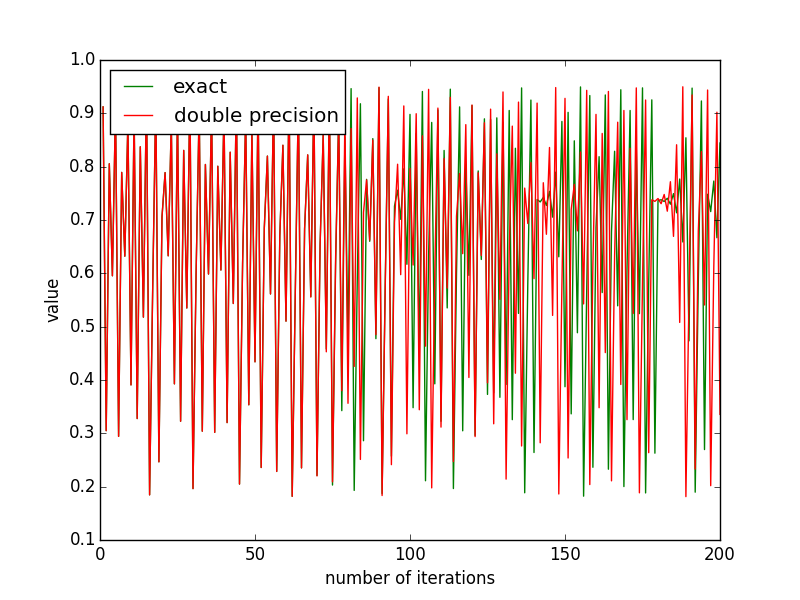
\includegraphics[width=0.9\textwidth]{logistic_map}
\end{frame}
\begin{frame}
  \frametitle{Logistic Map}
  \centering
  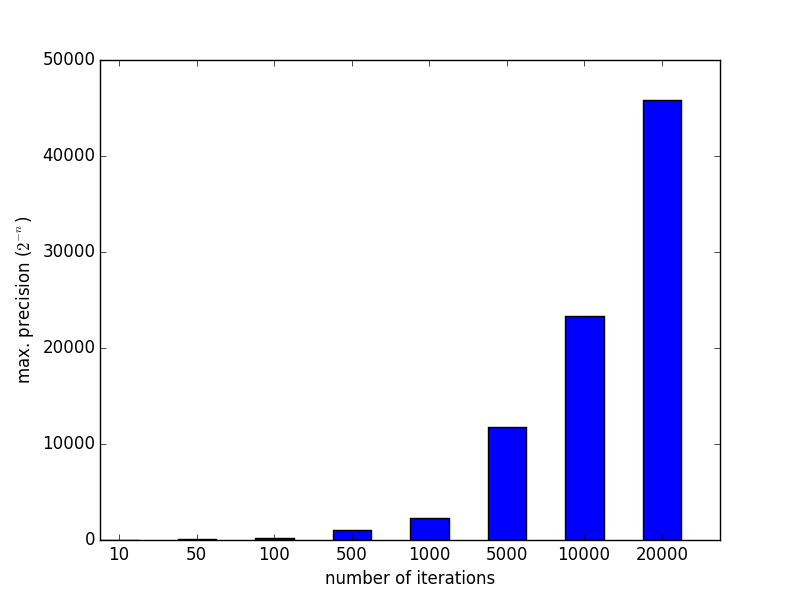
\includegraphics[width=0.9\textwidth]{logmap2}
\end{frame}
\begin{frame}
  \frametitle{Multivalued Functions}
  \large
  A multivalued function $f$ is allowed to have multiple valid outputs $f(x)$ for an argument $x$.
  \pause
  \vfill
  In practice, that means that the output may also depend on the internal representation of $x$
  and not only on the real number $x$.
  \pause
  \vfill
  The output of a multi-valued function can change from one iteration to another.
  To prevent a change of program flow, it is necessary to save the output of a multi-valued function (multi-valued cache).
\end{frame}
\begin{frame}
  \frametitle{Limits}
  \begin{itemize}[<+->]
    \item everything seen so far can also be done by symbolic computation.
    \item there is no need for computable analysis yet
    \item \irram also allows the user to define new real numbers and functions
  \end{itemize}
\end{frame}
\begin{frame}[<+->][fragile]
  \frametitle{Simple Limits}
  \begin{lstlisting}
  REAL limit (REAL f(int));
  \end{lstlisting}
  Defines a new \real from an algorithm to generate that real.
  \vfill
  \pause
  \begin{lstlisting}
  REAL limit (REAL a(int, const REAL&),
                      const REAL& x);
  \end{lstlisting}
  returns the value $f(x) = \lim_{n \to \infty} a(n,x)$.
  $a$ has to converge rapidly.
\end{frame}

\begin{frame}
	\begin{beamercolorbox}[sep=8pt,center,shadow=true,rounded=true]{title}
      \usebeamerfont{title}
	Case Study: A Data Type for Analytic Functions\par%
    \end{beamercolorbox}
\vfill
\end{frame}
\subsection{Analytic Functions}
\begin{frame}
\frametitle{Analytic Functions and Computational Complexity}
\begin{fact}
For general polynomial time computable functions, many important operators have been shown to be computationally hard.\\
For example
\pause
\begin{itemize}[<+->]
\item Polynomial time computable functions may have noncomputable derivatives. (Ko 1983)
\item Parametric maximization is NP-hard. (Ko/Friedman (1982))
\item Integration is \#P-hard. (Friedman (1984))
\end{itemize}
\end{fact}
\pause
We want to find a subset of polynomial time computable functions on which we can perform those operations in polynomial time.
\end{frame}
\begin{frame}
\frametitle{Analytic Function}
An analytic function is a function locally given by a complex power series.\\
\begin{definition}[Analytic Function]
% \begin{columns}
% \begin{column}{0.4\linewidth}
$f : D \to \C $, $D \subseteq \C$ is analytic if for any $x_0 \in D$ the Taylor-series
$$ T(x) := \sum^\infty_{n=0} a_n(x-x_0)^n$$
converges to $f(x)$ for $x$ in a neighborhood of $x_0$.  
% \end{column}
% \begin{column}{0.4\linewidth}
% \includegraphics[width=4.5cm]{TaylorComplexConv}
% \end{column}
% \end{columns}
\end{definition}
\end{frame}
\begin{frame}
\frametitle{Some non-uniform results}

$$a_m =\frac{f^{(m)}(x_0)}{m!} 
, \,\, f(x) = \sum_{m=0}^\infty a_m(x-x_0)^k \,\ \text{ for } x \in B(x_0,R)
$$
\vfill
\begin{theorem}[Pour-El, Richards, Ko, Friedman, M\"uller (1987/1989)]
$f$ is (polytime) computable iff $(a_m)_{m \in \N}$ is.
\end{theorem}
 \onslide<2->{
From that polynomial time computability of the derivative and the anti-derivative of a function follows immediately.
}
\end{frame}
\begin{frame}
\frametitle{Some non-uniform results}
$$a_m =\frac{f^{(m)}(0)}{m!} 
, \,\, f(x) = \sum_{m=0}^\infty a_mx^k \,\ \text{ for } x \in B(0,R)
$$
\vfill
\begin{theorem}[M\"uller (1995)]
\begin{itemize}
\item The operator $f \to (a_m)_{m \in \N}$ is not computable.
\item The evaluation operator $((a_m)_{m \in \N},x) \to f(x) $ is not computable.
\end{itemize}
\end{theorem}
\pause
However, if we supply some additional (discrete) information those operators become computable.
\end{frame}


\subsection{Representing power series}
\begin{frame}
\frametitle{A practical representation for power series}
\begin{lemma}
  Let $f : [0,1] \to \C$ be real analytic.\\
  Then there exists an $l \in \N$ such that 
  $$ \forall x \in [0,1]: \, \left | \frac{f^{(j)}(x)}{j!} \right | \leq 2^l\cdot l^j $$
\end{lemma}
\pause
$l$ can be used to make a tail estimate on
$$ \left | \sum_{n \geq N} a_m z^n \right |  $$
\end{frame}
%\begin{frame}
%\frametitle{Finding $k$ and $A$}
%\begin{itemize}
%\item Choose $k$ appropriately and let $r := \sqrt{k}{2}$
%\item $f_{|z|=r}$ is a continuous function on a compact domain, thus is bounded by some number $A$
%\item By Cauchy Differentiation formula $$|a_n| \leq |\frac{1}{2\pi i}\int_{z=|r|} \frac{f(z)}{|z|^{n+1}} d \lambda| \leq \frac{A}{r^n}$$
%\end{itemize}
%\end{frame}
\begin{frame}[<+->]
\frametitle{Analytic Functions and Computational Complexity}
\begin{theorem}[Kawamura, R\"osnick, M\"uller, Ziegler (2013)]
  The following operators are computable in time polynomial in $k+l$, where $2^{-n}$ is the output precision.
\begin{enumerate}
\item evaluation
\item addition and multiplication
\item differentiation and anti-differentiation
\item parametric maximization
\end{enumerate}
\end{theorem}
\end{frame}
\begin{frame}
\frametitle{Analytic Continuation}
\begin{minipage}{0.45\textwidth}
\begin{center}
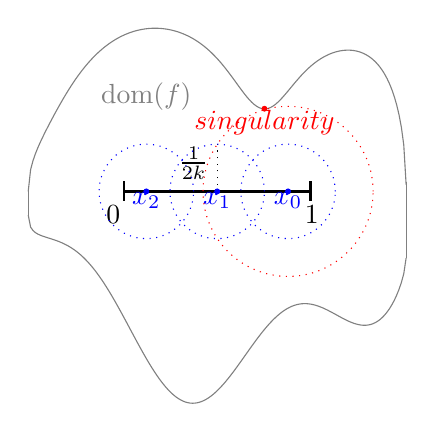
\begin{tikzpicture}[scale=0.6]
%    \draw<3> (-1,1) rectangle (5,-1);
    \node<1->  at (-0.2,-0.5) {$0$};
    \node<1->  at (4.0,-0.5) {$1$};
    \draw<1-> [thick,|-|] (0,0) -- (4,0);
    \node<2->  at (1.5,.6) {$\frac 1{2k}$};
    \draw<2->  [dotted] (2.0,0) -- (2.0,1);
    \draw<1-> [domain = 0:8,color=gray] plot[samples=160] (\x-2, {sqrt(16-(\x-4)^2)*(1-1/(\x^2+1) + sin(\x) + (\x/7)^5-\x/6 +1.5- 1/((\x-5)^2+1))/2});
    \draw<1-> [domain = 0:8,color=gray] plot[samples=160] (\x-2, {1/(\x^2+1)/2 + sin(80*\x) + (\x/7)^5-\x/6 -1-sqrt(16-(\x-4)^2)/2});
    \draw<1-> [color=gray] (-2,0) -- (-2,-.5);
    \draw<1-> [color=gray] (6,.19) -- (6,-1.42);
    \node<1-> [color=gray] at (.5,2) {$\dom(f)$};
    \draw<2-> [fill=blue,radius =.05,color=blue] (3.5,0) circle;
    \node<2-> [color=blue] at (3.5,-.2) {$x_0$};
    \draw<2-> [fill=blue,radius =.05,color=blue] (2.0,0) circle;
    \node<2-> [color=blue] at (2.0,-.2) {$x_1$};
    \draw<2-> [radius = 1,color=blue, dotted] (2.0,0) circle; 
    \draw<2-> [fill=blue,radius =.05,color=blue] (0.5,0) circle;
    \node<2-> [color=blue] at (0.5,-.2) {$x_2$}; 
    \draw<2-> [radius = 1,color=blue, dotted] (0.5,0) circle;
    \draw<2-> [radius = 1,color=blue, dotted] (3.5,0) circle;
    \draw<2-> [radius = 1.8, color = red, dotted] (3.5,0) circle; 
    \draw<1-> [fill=red,radius = .05,color = red] (3,1.75) circle;
    \node<1-> [color=red] at (3,1.45) {$singularity$};
\end{tikzpicture}
\end{center}
\end{minipage}
\hfill
\begin{minipage}{0.45\textwidth}
  \onslide<3>{
  The function is uniquely defined by a single germ, i.e., the sequence
  $(\frac{f^{(j)}(x_0)}{j!})_{j \in \N}$ for some $x_0 \in [0,1]$
}
\end{minipage}
\end{frame}

\begin{frame}
\frametitle{Analytic Continuation}
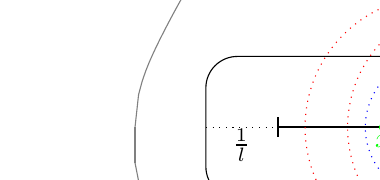
\begin{tikzpicture}[scale=0.9]
    \path [use as bounding box,red] (-100pt,-10pt) rectangle (30pt,40pt);
    \draw[rounded corners=4mm] (-1,1) rectangle (5,-1);
    %\draw (2,0) ellipse (3cm and 1cm);
    \draw [thick,|-|] (0,0) -- (4,0);
    \node at (-.5,-.25) {$\frac 1l$};
    \draw [dotted] (-1,0) -- (0,0);
    \node at (2.2,.5) {$\frac 1l$};
    \draw [dotted] (2,1) -- (2,0);
    \draw [domain = 0:8,color=gray] plot[samples=160] (\x-2, {sqrt(16-(\x-4)^2)*(1-1/(\x^2+1) + sin(\x) + (\x/7)^5-\x/6 +1.5- 1/((\x-5)^2+1))/2});
    \draw [domain = 0:8,color=gray] plot[samples=160] (\x-2, {1/(\x^2+1)/2 + sin(80*\x) + (\x/7)^5-\x/6 -1-sqrt(16-(\x-4)^2)/2});
    \draw [color=gray] (-2,0) -- (-2,-.5);
    \draw [color=gray] (6,.19) -- (6,-1.42);
    \node [color=gray] at (.5,2) {$\dom(f)$};
    \draw<1-3> [fill=blue,radius =.05,color=blue] (3.5,0) circle;
    \node<1-3> [color=blue] at (3.5,-.2) {$x_0$};
    \draw<1-3> [radius = 1,color=blue, dotted] (3.5,0) circle;
    \draw<1-3> [radius = 1.8, color = red, dotted] (3.5,0) circle; 
    \node<2> [color=red] at (2.5,-5) {Check if $x$ in circle};
    \draw [fill=green, radius = .05, color = green] (1.5,0) circle;
    \node [color=green] at (1.5,-.2) {$x$};
    \node<3> [color=red] at (3.0,-5) {Compute Taylor coefficients around $x_1$};
    \draw<3-5> [fill=cyan, radius = .05, color = cyan] (2.75,0) circle;
    \node<3-5> [color=cyan] at (2.75,-.2) {$x_1$};
    \draw<3-5> [radius = 1,color=cyan, dotted] (2.75,0) circle;
    \draw<4-5> [radius = 1.75, color = red, dotted] (2.75,0) circle; 
    \node<4> [color=red] at (2.5,-5) {Check if $x$ in circle};
    \node<5> [color=red] at (3.0,-5) {Compute Taylor coefficients around $x_2$};
    \draw<5-6> [fill=blue, radius = .05, color = blue] (2.25,0) circle;
    \node<5-6> [color=blue] at (2.25,-.2) {$x_2$};
    \draw<5-6> [radius = 1,color=blue, dotted] (2.25,0) circle;
    \draw<6> [radius = 1.85, color = red, dotted] (2.25,0) circle; 
\end{tikzpicture}
\end{frame}
\begin{frame}[<+->]
\frametitle{Computing Taylor coefficients}
\begin{itemize}
  \item The coefficients around some new point $x_0 \in [0,1]$ are given by $c_j := \frac{f^{(j)}(x_0)}{j!}$
  \item $\frac{f^{(d)}(x_0+z)}{d!} = \sum_{j=0}^\infty c_{j+d}\cdot {j+d \choose d}\cdot z^j$
  \item $\left | \sum_{j \geq J} c_{j+d}\cdot {j+d \choose d}\cdot z^j \right | \leq l^d\cdot 2^{l+1-J}(d+1)\cdot {J+d \choose d}$
\end{itemize}
\end{frame}


\subsection{Implementation}
\begin{frame}[<+->]
\frametitle{Implementation}
\begin{itemize}
    \item A data type for functions real analytic on $[0,1]$ was implemented in \irram .
    \item Constructor from a single power series.
    \item Analytic continuation used if more series are needed to cover the interval. 
    \item The running time and memory usage was empirically analyzed.
    \item Running time increases quickly with number of analytic continuations. 
\end{itemize}
\end{frame}
\begin{frame}[t]{Riemann Mapping Theorem}
  \begin{theorem}[Riemann]
    Let $U \subsetneq \C$ be non empty, simply connected and open.\\
    Then there exists a biholomorphic mapping from $U$ on to the open unit disc.
%\begin{tikzpicture}[scale=0.9]
%    \path [use as bounding box,red] (-100pt,-10pt) rectangle (30pt,40pt);
%    \draw (-3,0.5) rectangle (2,-0.5);
%    \draw [thick,->] (2.2,0) -- (3.8,0);
%    \draw (5,0) ellipse (1cm and 1cm);
%\end{tikzpicture}
  \end{theorem}
\vfill \pause
 How complex is it to compute this mapping?\\
  \pause
  In the general case $\#P$ hard (Binder, Braverman, Yampolsky).\\
  \pause
  Riemann mappings of domains with polynomial time computable analytic boundaries are polynomial time computable (Rettinger).
\end{frame}
\begin{frame}[<+->]{Summary}
 When developing Exact Real Arithmetic algorithms the following is important
 \begin{itemize}
     \item Careful mathematical analysis of the errors that arise by finite approximations has to be performed.
     \item Theorems from real and complex analysis have to be combined with methods from theoretical computer science to get efficient algorithms.
     \item Finding the right restriction of the type of functions considered, so that efficient algorithms are possible but the class still contains most functions relevant in practice.
     \item It is sometimes necessary to enrich the input by natural parameters of the function to gain better computability or complexity results.
 \end{itemize}
\end{frame}

\begin{frame}
	\begin{beamercolorbox}[sep=8pt,center,shadow=true,rounded=true]{title}
      \usebeamerfont{title}
	Future Work\par%
    \end{beamercolorbox}
\vfill
\end{frame}
\subsection{Future}
\begin{frame}
\frametitle{Future Work}
\begin{itemize}
    \item Extend class for analytic functions to multi dimensional case
    \item Solver for ODEs with analytic right hand sides
    \item Detailed Analysis of Numerical ODE solvers
	\item Parametrized analysis of such approaches will be performed
	\item taking into account the number of steps and the intermediate precision required to attain guaranteed
output error $2^{-n}$
\end{itemize}
\end{frame}

\begin{frame}

    \vspace{\fill}
\begin{beamercolorbox}[center,shadow=true,rounded=true]{note} 
        \huge Thank you!
\end{beamercolorbox}

    \vspace{\fill}
\end{frame} 
{
\makeatletter % to change template
    \setbeamertemplate{headline}[default] 
    \def\beamer@entrycode{\vspace*{-\headheight}} 
\makeatother
\begin{frame}{References}
\fontsize{6pt}{7.2}\selectfont 
\nocite{*}
\def\newblock{}
\bibliographystyle{abbrv}

\begin{thebibliography}{10}   

  \beamertemplatearticlebibitems
  \bibitem{6}
	Harvey Friedman,
    \newblock \emph{ The computational complexity of maximization and integration}, Adv. in Math. 53 (1984), no. 1, 80-98. MR 748898 (86c:03037)
  \beamertemplatearticlebibitems
  \bibitem{1}
	Akitoshi Kawamura, Norbert Th. M\"{u}ller, Carsten R\"{o}snick, and
Martin Ziegler
    \newblock \emph{Parameterized Uniform Complexity in Numerics:
from Smooth to Analytic, from NP-hard to Polytime}, pre-print (2012).

  \beamertemplatearticlebibitems
  \bibitem{7}
	Ker-I Ko,
    \newblock \emph{ Complexity theory of real functions}, Progress in Theoretical Computer Science, Birkh\"{a}user Boston Inc., Boston, MA, 1991.
MR 1137517 (93i:03057)

  \beamertemplatearticlebibitems
  \bibitem{8}
	Ker-I Ko,
    \newblock \emph{  On the Computational Complexity of Ordinary Differential Equations}, Information and Control 58(1-3): 157-194 (1983)


  \beamertemplatearticlebibitems
  \bibitem{2}
	Norbert Th. M\"{u}ller,
    \newblock \emph{ The \irram: Exact Real Arithmetic in C++}, Computability and Complexity in Analysis (2000) .

  \beamertemplatearticlebibitems
  \bibitem{Mul95}
	Norbert Th. M\"{u}ller,
    \newblock \emph{ Constructive aspects of analytic functions}, Computability
and Complexity in Analysis (Ker-I Ko and Klaus Weihrauch, eds.),
Informatik Berichte, vol. 190, FernUniversit\"{a}t Hagen, September
1995, CCA Workshop, Hagen, August 19-20, 1995, pp. 105-114.

  \beamertemplatearticlebibitems
  \bibitem{4}
	Norbert Th. M\"{u}ller,
    \newblock \emph{ Uniform Computational Complexity of Taylor Series}, ICALP 1987: 435-444

  \beamertemplatearticlebibitems
  \bibitem{5}
	Norbert Th. M\"{u}ller,
    \newblock \emph{ Polynomial Time Computation of Taylor Series}, Proc. 22 JAIIO - PANEL 1993

  \beamertemplatearticlebibitems
  \bibitem{9}
	Marian B. Pour-El and J. Ian Richards,
    \newblock \emph{ Computability in analysis
and physics}, Perspectives in Mathematical Logic, Springer-Verlag,
Berlin, 1989. MR 1005942 (90k:03062)
  \beamertemplatearticlebibitems
  \bibitem{11}
	Florian Steinberg,
    \newblock \emph{A type of Taylor series for the C++ library iRRAM for exact real arithmetic} (draft) last edited November 28, 2013
  \beamertemplatearticlebibitems
  \bibitem{10}
	Klaus Weihrauch,
    \newblock \emph{Computable analysis}, Texts in Theoretical Computer
Science. An EATCS Series, Springer-Verlag, Berlin, 2000, An
introduction. MR 1795407 (2002b:03129)

  \end{thebibliography}

\end{frame}
}
\end{document}
